\IEEEPARstart{A} utomatic action recognition, in videos, has caught an extensive research interest recently, 
in computer vision, mostly due to its wide range of real world applications, such as, 
sport applications, health care, video surveillance, robot vision, human-computer interaction
etc. Furthermore, with the rapid growth of digital video data, in modern world, 
the need for automatic
classification and indexing of video data, has become vital than ever. 

\tikzset{
  font={\fontsize{4pt}{5}\selectfont}}
    




\begin{figure}
  \centering
  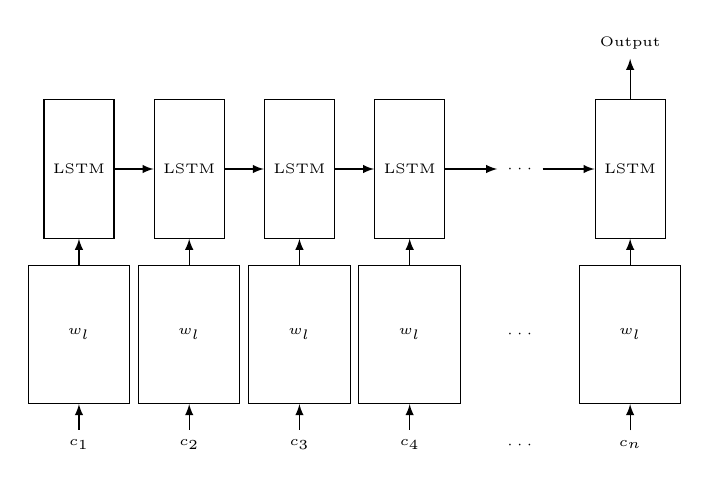
\begin{tikzpicture}[x=0.7cm, y=0.7cm] 
	\foreach \i/\l in {1/1, 2/2, 3/3, 4/4, 6/n}
	{
		\node[draw=black, minimum height=50] (1\i) at (2*\i, 0) {LSTM};
		\node[draw=black, minimum height=50, text width=30, align=center] (2\i) at (2*\i, -3) {$w_l$};
		\node[text width=30, align=center] (3\i) at (2*\i, -5) {$c_\l$};		
	}
	
	\node (15) at (2*5,0) {$\cdots$};
	\node (25) at (2*5,-3) {$\cdots$};
	\node (35) at (2*5,-5) {$\cdots$};	
	
	\foreach  \i/\j in {1/2, 2/3, 3/4, 4/5, 5/6}
	{
		\draw [-latex] (1\i) -- (1\j);
	}
	
	\foreach  \i in {1,2,3,4,6}
	{
		\draw [-latex] (2\i) -- (1\i);
		\draw [-latex] (3\i) -- (2\i);
	}	
	
	\draw[-latex] (16) -- +(0,2) node [anchor=south] {Output};
	

\end{tikzpicture}
  \caption{Test Figure}\label{fi:test1}
\end{figure}



Despite the increasing interest, in this field, state-of-the-art
systems are still far from human performance, in contrast to image classification \cite{girshick2014rich},
 \cite{krizhevsky2012imagenet}. This is
partially due to the fact that, videos in nature, consist of complex intra-class variations. Some
obvious causes behind this dilemma are, variability of the view point change, background 
clutter, high dimensionality of data, lack of larger datasets, and low resolution. 

But, despite the fact, that most of these issues, up to some extent, also exists in 
automatic image classification, it has achieved immense success, in recent years,
largely owing to the rise of deep learning techniques. Therefore, it is worth to investigate,
what is holding back video classification, and find solutions. In this study, mainly, three such key
areas are addressed.

A complex activity is typically composed of several sub activities. 
But, most of the existing accomplished approaches, try to classify a video, treating it as a 
single, high level activity \cite{wang2011action}, \cite{wang2013action}, \cite{simonyan2014two}, 
\cite{7486474}.
As the action becomes complex, the behavior, and the 
temporal evolution of its underlying sub events, becomes more complicated. For example,
cooking may involve sub actions: cutting, turning on cooker, stirring etc. They may not always preserve this 
same low level order, for same action class. Rather, they may contain 
a higher order temporal relationship among them. For example, turn on cooker and cutting,
may change the order in another video in the same class. 
Therefore, this temporal pattern of sub events, is not easy to capture through a simple
time series analysis. These patterns can only be identified, by observing a large number
of examples, using a system, which as an infinite dynamic response. Therefore, we argue that, it is critically important to
model this higher order temporal
progression, and capture temporal dynamics of these sub events, for better recognition of
complex activities. 

Recognition accuracy of a complex activity, largely depends on the recognition accuracy 
of underlying sub events. In contrast to image classification, the information contained in videos, 
are not 
 in a single domain. Both, the motion patterns of the actors and objects, as well as the static
 information, such as, background, interactive/still objects, are important for determining an action.
For example, the body movements of a group of people fighting, may closely relate with 
body movements of a sports event. In such a case, it is tough to distinguish between the two 
activities, solely by looking at the motion patterns. Inspecting the background setting, 
and objects are crucial in such a scenario. Therefore it is necessary to engineer powerful features,
from both motion and static domains. In addition, these features must be complementary, and one feature domain should 
not influence other domain. In other words, they should be self explanatory, and mutually exclusive, to an utmost level. 
Also, these motion features should be able to capture
activities of each actor independently, so later, the distributional properties of these actions, over shorter 
and longer time ranges, can be used to identify high level actions. In this proposed method, such a feature crafting mechanism, is provided. 

Furthermore, how to combine these descriptors, in two different domains, remains a key challenge.
The combined descriptor, should contain the essence of both domains, and should not have a 
negative interference on each other. Recently, there has been attempts to answer this aspect \cite{7486474},\cite{simonyan2014two}. 
One major requirement, is to 
have a high level intuitive interpretation, on how much contribution does each domain provide to the 
final descriptor, and have the authority to control that contribution, in which, we put 
our special focus. This makes it possible 
to deeply investigate the the contribution of each domain, for a better accuracy. 

In this work, we focus specially on the problematic areas, mentioned above, and provide 
novel and efficient methods to overcome these issues. In order to examine the temporal evolution 
of sub activities later, we create video segments with constant overlap. Afterwards, static and motion
descriptors are engineered to represent each segment. We propose \textbf{motion tubes},
a dense trajectory \cite{wang2011action} based tracking mechanism, to identify and track candidate moving areas, 
separately. This enables independent modeling of the activities, in each moving area.
In order to capture motion patterns proficiently, histogram oriented optic flows (HOOF) \cite{chaudhry2009histograms}
, are used, inside motion tubes. Then, a bag of words method is applied on the generated 
features, to capture the distributional properties of micro actions, and create high level, discriminative motion features. 

Inspired by the power of CNNs, in the task of object recognition, we create a 7 layer deep
convolutional neural net, and pre-train in on the popular Imagenet dataset \cite{deng2012imagenet}.
Afterwards, this trained CNN is used to create deep features, which are used for creating static descriptors. 

Then, a computationally efficient, yet powerful mathematical model is proposed to fuse these 
two feature vectors. This model provides the ability, to control the contribution of each domain,
to the final fused discriptor. Therefore, utilizing this intuition, we investigate the 
optimum contribution of each domain, for a better accuracy, and solidly justify that, these 
features are complementory, and contribute to the final accuracy. 

In order to model the temporal progression of sub events, the fused vectors are then fed to 
a LSTM network, where, underlying temporal patterns of the sub events are discovered, and high level actions 
are classified. We feed the same vectors to a classifier, which does not capture temporal dynamics,
and show that, modeling temporal progression of sub events, indeed contribute for a better 
accuracy. 

We carry out our experiments on the two popular action datasets, UCF-11 \cite{liu2009recognizing}
and Hollywood2 \cite{marszalek2009actions}. Our results exceeds existing best state-of-the-art
results on these datasets, to the best of our knowledge.

The key contributions of this paper, can be summarized as follows:

 \begin{itemize}
  \item We propose an end to end system, which simultaneously extracts static and motion information, fuse, and models the 
temporal evolution of sub activities, and does action classification. 
  \item We propose a novel, moving actor/object tracking mechanism, called \textit{motion tubes},
which enables the system to track each actor/object independently, and model the motion patterns individually. 
This allows the system to model actions, occurring in a video, in micro level, and utilize these learned dynamics
at a high level, afterwards.
 \item We propose a novel, simple and an efficient mathematical model for fusioning two vectors, 
in two different 
domains, based on Choleskey transformation. This method provides the ability to govern the contribution of each domain,
for the fused vector, precisely in exact numbers, rather than empirically. Utilizing this advantage, we prove that,
both static and motion information are complementary and vital for activity recognition, through experiments.
  \item We model the underlying 
temporal evolution of sub events, for complex action recognition, using a LSTM network. Through our experiments,
we prove that, capturing these dynamics, indeed benefits the final accuracy. 
\item With the proposed technique, and novel techniques,
we outperform the existing best results for the popular datasets UCF-11 \cite{liu2009recognizing}
and Hollywood2 \cite{marszalek2009actions}.
 \end{itemize}




